% !TeX spellcheck = de_AT_frami
\section{Lineare Algebra}
	\begin{enumerate}
		\item \textbf{Wie ist die LU-Zerlegung definiert?} \\
			Es sei A eine invertierbare \(n\times n\)-Matrix. Dann existieren drei ebenfalls invertierbare Matrizen und zwar eine Permutationsmatrix P, eine untere Dreieckmatrix L und eine obere Dreiecksmatrix U, d.h.
			\begin{align*}
				L = \begin{bmatrix}
					1 & 0 & \dots & 0 \\
					\ell_{21} & \ddots & \ddots & \vdots \\
					\vdots & \ddots & \ddots & 0 \\
					\ell_{n1} & \dots & \ell_{n,n-1} & 1
				\end{bmatrix}, \quad
				U = \begin{bmatrix}
					u_{11} & u_{12} & \dots & u_{1n}\\
					0 & \ddots & \ddots & \vdots \\
					\vdots & \ddots & \ddots & u_{n-1,n} \\
					0 & \dots & 0 & u_{nn}
				\end{bmatrix}
			\end{align*}
			mit \(u_{ii}\neq0,\,i=1,\dots,n\), sodass
			\begin{align*}
				PA=LU
			\end{align*}
			gilt. Diese Zerlegung heißt LU-Zerlegung. Die Multiplikation mit P von links entspricht einer Vertauschung der Zeilen von A wegen der Spaltenpivotsuche.
		
		\item \textbf{Was bedeutet Spaltenpivotsuche und wieso wird sie verwendet?} \\
			Für die LU-Zerlegung wählt man das betragsmäßig größte Element der Pivotspalte als Pivotelement. Dieser Vorgang wird als Spaltenpivotsuche bezeichnet. \\
			Im \(k\).ten Schritt der LU-Zerlegung heißt dies: Suche das betragsgrößte Element in der \(k\)-ten Spalte in den Zeilen \(k,k+1,\dots,n\)!
		
		\item \textbf{Wie erhält man die Permutationsmatrix bzw. den Permutationsvektor?} \\
			Permutationsmatrix P
			\begin{itemize}
				\item Starte mit der Einheitsmatrix
				\item Führe an dieser Matrix ebenfalls die entsprechend der Pivotsuche beim Gaußschen Algorithmus notwendige Zeilenvertauschung durch.
			\end{itemize}
			Permutationsvektor IP mit Länge \(n\)
			\begin{itemize}
				\item \(\text{IP}[n]=(-1)^{\text{Anzahl Vertauschungen}}\)
				\item \(\text{IP}[k]=m\) \\
					Im \(k\)-ten Eliminationsschritt wird die Zeile \(m\) mit der aktuellen Zeile \(k\) vertauscht.
				\item Alternativ: Man erstellt Vektor \(\begin{bmatrix}
				1 & 2 & \cdots & n
				\end{bmatrix}^\text{T}\) und wendet darauf die Vertauschen an.
			\end{itemize}
		
		\item \textbf{Wie löst man die LU-Zerlegung lineare Gleichungssysteme \(\mathbf{AX=b}\)?} \\
			\begin{enumerate}
				\item[Schritt 1:] Vertauschen der Elemente von b mit Hilfe von IP \(\Rightarrow\tilde{\text{b}}\)
				\item[Schritt 2:] Vorwärtssubstitution mit L und \(\tilde{\text{b}}\) \\
				\(\text{Ly}=\tilde{\text{b}}\Rightarrow\text{y}\)
				\item[Schritt 3:] Rückwärtssubstitution mit U und y \\
				\(\text{Ux=y}\Rightarrow \text{x}\)
			\end{enumerate}
		
		\item \textbf{Wie berechnet man \(\mathbf{\det A}\) mit Hilfe der LU-Zerlegung?}
			\begin{align*}
				\det{A}=u_{11}\cdot u_{22}\cdots u_{nn}\cdot\text{IP[n]}
			\end{align*}
		
		\item \textbf{Wie groß ist der Rechenaufwand der LU-Zerlegung und für das Auflösen eines linearen Gleichungssystems?}
			\begin{itemize}
				\item LU-Zerlegung: \(\frac{n^3}{3}+\mathcal{O}(n^2) \quad\) \text{Operationen}
				\item Auflösen l.Gls.: \(n^2+\mathcal{O}(n) \quad\) Operationen
			\end{itemize}
		
		\pagebreak
		
		\item \textbf{Wie ist die Cholesky-Zerlegung einer Matrix A definiert? Welche Eigenschaften muss A besitzen?} \\
			Cholesky-Zerlegung: A=CC\(^\text{T}\) wobei der Cholesky-Faktor C eine untere Dreiecksmatrix von A ist. \\
			Eigenschaften die A haben muss:
			\begin{itemize}
				\item reell: Die Koeffizienten von A sind reelle Zahlen;
				\item symmetrisch: \(\text{A}=\text{A}^\text{T}\);
				\item positiv definit: Für alle \(x\neq0\) gilt \(x^\text{T}Ax>0\).
			\end{itemize}
		
		\item \textbf{Wie berechnet man die Cholesky-Zerlegung?} \\
			Für alle Spalten \(k=1,\dots,n\) von links beginnend:
			\begin{itemize}
				\item[] Diagonalelement \(c_{kk}=\sqrt{a_{kk}-c_{k1}^2-\cdots-c_{k,k-1}^2}\)
				\item[] Für alle Elemente \(c_{ik},i>k,\) also unterhalb von \(c_{kk}\):\\
				\mbox{}\hspace{0.5cm}\(c_{ik}=(a_{ik}-c_{i1}c_{k1}-\cdots-c_{i,k-1}c_{k,k-1})/c_{kk}\)
			\end{itemize}
		
		\item \textbf{Wie groß ist der Rechenaufwand einer Cholesky-Zerlegung?} \\
			\(\frac{n^3}{6}+\mathcal{O}(n^2)\), Hälfte der LU-Zerlegung dank Symmetrie von A.
		
		\item \textbf{Wie löst man mit der Cholesky-Zerlegung lineare Gleichungssysteme \(\mathbf{Ax=b}\)?}
			\begin{align*}
				\text{Ax}=\text{b}&\Longleftrightarrow \text{C}\underbrace{\text{C}^\text{T}\text{x}}_\text{y}=\text{b} \\
				\text{Cy}&=\text{b} \Rightarrow \text{y} \\
				\text{C}^\text{T}\text{x}&=\text{y} \Rightarrow \text{x}
			\end{align*}
		
		\item \textbf{Wie ist die rationale Cholesky-Zerlegung einer Matrix A definiert? Welche Eigenschaften muss A besitzen?}
			\begin{align*}
				\text{A}=\text{LDL}^\text{T}
			\end{align*}
			Wobei L eie untere Dreiecksmatrix mit Einsen in der Diagonale und D eine Diagonalmatrix mit \(d_{ii}\neq0\) ist.\\
			A muss invertierbar und symmetrisch sein.
		
		\item \textbf{Wie berechnet man die rationale Cholesky-Zerlegung?} \\
			
		
		\item \textbf{Wie löst man mit der rationalen Cholesky-Zerlegung lineare Gleichungssysteme \(\mathbf{Ax=b}\)?}
			\begin{align*}
				\text{Ax}=\text{b}&\Longleftrightarrow \text{LDL}^\text{T}\text{x}=\text{b}
			\end{align*}
		
		\item \textbf{Wie ist die Matrixnorm allgemein definiert?} \\
			Gegeben sei ein Vektorraum \(V\). Eine Norm \(V\) ist eine Abbildung \(||\cdot||:V\rightarrow\mathbb{R}\) mit den folgenden Eigenschaften:
			\begin{itemize}
				\item[(i)] \(||x||\geq 0,\quad ||x||=0\Rightarrow x=0\),
				\item[(ii)] \(||\lambda x||=|\lambda|\cdot||x||\),
				\item[(iii)] \(||x+y||\leq||x||+||y||\). (Dreiecksungleichung)
			\end{itemize}
		
		\pagebreak
		
			\item \textbf{Wie berechnet man \(\mathbf{||\text{A}||_1}\), \(\mathbf{||\text{A}||_2}\) und \(\mathbf{||\text{A}||_\infty}\) ?} \\
			\begin{itemize}
				\item Es sei A eine \(m\times n\)-Matrix.
					Die Matrixnorm für die 1-Norm
					\begin{align*}
						||\text{A}||_1=\underset{1\leq j\leq n}{\max}\left( \sum_{i=1}^{m}|a_{ij}|\right) 
					\end{align*}
					ist die maximale Spaltenbetragssumme. Merkregel: 1 steht wie eine Spalte.
				\item Die Matrixnorm für die \(\infty\)-Norm
					\begin{align*}
						||\text{A}||_\infty=\underset{1\leq i\leq m}{\max}\left( \sum_{j=1}^{n}|a_{ij}|\right)
					\end{align*}
					ist die maximale Zeilenbetragssumme. Merkregel: \(\infty\) liegt wie eine Zeile.
				\item Die Matrixnorm für die 2-Norm (euklidische Norm):
					\begin{align*}
						||\text{A}||_2=\sqrt{\text{größter Eigenwert von A}^\text{T}\text{A}}
					\end{align*}
			\end{itemize}		
			
		\item \textbf{Wie ist die Norm von \(\mathbf{A^{-1}}\) definiert?} \\
			\begin{align*}
				||\text{A}^{-1}||:=\left(\underset{x\neq0}{\text{inf}}\frac{||\text{Ax}||}{||\text{x}||}\right)^{-1} = \left(\underset{||\text{y}||=1}{\text{inf}}||\text{Ay}||\right)^{-1}
			\end{align*}
		
		\item \textbf{Wie ist die Kondition einer linear Abbildung bzw. einer Matrix A definiert?}
			\begin{align*}
				\kappa(\text{A}):=||\text{A}||\cdot||\text{A}^{-1}||
			\end{align*}
		
		\item \textbf{Was gilt für den relativen Fehler der Lösung eines linearen Gleichungssystems?}
			\begin{align*}
				\frac{||\tilde{\text{x}}-\text{x}||}{||\text{x}||}\leq \frac{\kappa(\text{A})}{1-\varepsilon_\text{A}\cdot\kappa(\text{A})}(\varepsilon_\text{A}+\varepsilon_\text{b})
			\end{align*}
		
		\item \textbf{Welche Eigenschaften besitzt die Kondition einer Matrix?}
			\begin{enumerate}
				\item[(1)] \(\kappa(\text{A})\geq1\).
				\item[(2)] Für \(\alpha\neq0\) ist \(\kappa(\alpha\text{A})=\kappa(\text{A})\)
				\item[(3)] \(\kappa(\text{A})=\frac{\sup_{||y||_2=1}||\text{Ay}||_2}{\inf_{||y||_2=1}||\text{Ay}||_2}=
				\frac{\sqrt{\lambda_{\max}}}{\sqrt{\lambda_{\min}}}\)
			\end{enumerate}
		
		\item \textbf{Welche Matrizen haben eine große/kleine Kondition?} \\
			Groß: Hilbertmatrix, Vandermonde-Matrix \\
			Klein: \(\text{A}=\alpha\text{I}, \quad \kappa(\text{A})=\kappa(\alpha\text{I})=\kappa(\text{I})=1\)\\
			\mbox{}\hspace{0.88cm} Für eine orthogonale Matrix Q gilt \(\kappa_2(\text{Q})=1\)
		
		\item \textbf{Was ist die Kondition der Einheitsmatrix?}
			\begin{align*}
				\kappa(\text{I})=1
			\end{align*}
		
		\pagebreak
		
		\item \textbf{Wie lässt sich die Kondition einer Matrix geometrisch interpretieren?} \\
			Verzerrungsfaktor:
			Es sei \(\varepsilon=\left\lbrace \text{A}\cdot\text{y}:||\text{y}||_2=1 \right\rbrace \) jene Ellipse, die durch Anwendung der Matrix auf A auf alle Vektoren mit Länge 1 erzeugt wird. Dann gilt:
			\begin{center}
				\(\kappa(\text{A}) \) = Umkreisradius/Inkreisradius der Ellipse \(\varepsilon\) = Verhältnis der Hauptachsen von \(\varepsilon\) = Verzerrungsfaktor von A.
			\end{center}
			\begin{figure}[htbp]
				\centering
				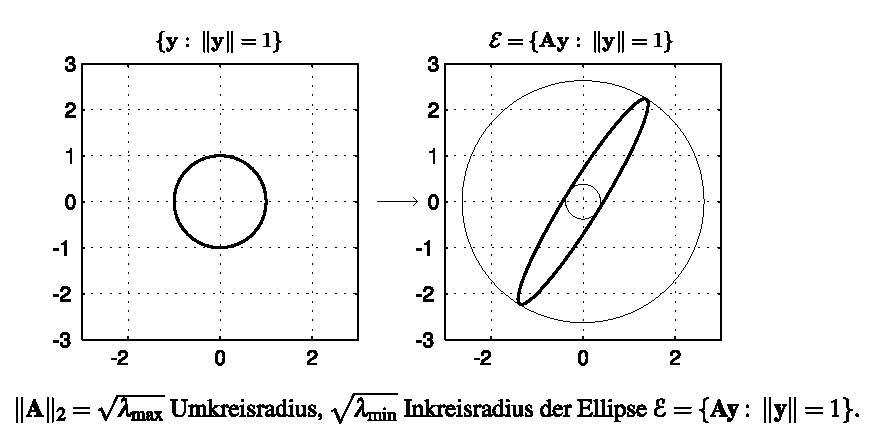
\includegraphics[width=0.6\linewidth]{kap5_1}
			\end{figure}
		
		
		\item \textbf{Wie lässt sich die Kondition eines linearen Gleichungssystems geometrisch interpretieren?} \\
			Eine Störung von b in einem Ax=b System verschiebt die erste Gerade leicht. Die neue Lösung eines gut Konditionierten Problems liegt wie in der Abbildung zu sehen näher an einer ungestörten Lösung als die eines schlecht Konditionierten.
			\begin{figure}[htbp]
				\centering
				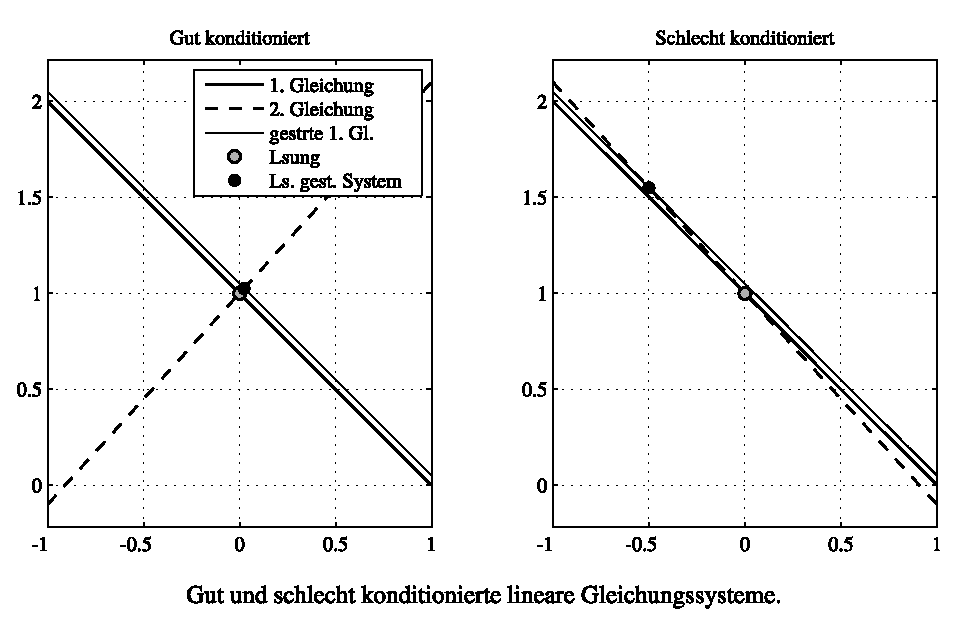
\includegraphics[width=0.6\linewidth]{kap5_2}
			\end{figure}
		
		\item \textbf{Wie ist die QR-Zerlegung definiert? Wozu wird sie verwendet?} \\
			Es sei A eine \(m\times n\)-Matrix mit \(m\geq n\) und \(\text{Rg}\,\text{A} = n\). Dann existiert eine orthogonale \(m \times m\)-Matrix Q mit
			\begin{align*}
				\text{A}=\text{QR}\quad \text{und} \text{R}=\begin{bmatrix}
					r_{11} & \cdots & r_{1n} \\
					 & \ddots & \vdots \\
					 0 & & r_{nn} \\
					 0 & \cdots & 0 \\
					 \vdots & & \vdots \\
					 0 & \cdots & 0 
				\end{bmatrix}.
			\end{align*}
			Die \(m \times n\)-Matrix R besteht aus einer oberen \(n\times n\)-Dreiecksmatrix und einem \((m-n)\times n\) Block aus Nullen darunter. Die Diagonalelemente \(r_{ii}\) sind alle von Null verschieden. \\
			QR-Zerlegung wird verwendet um überbestimmte lineare Gleichungssysteme im Sinne der kleinsten Fehlerquadrate zu lösen.
		
	\end{enumerate}